\documentclass[a4paper]{article}
\setlength{\parindent}{0pt}

%%%%%%%% CREATE DOCUMENT STRUCTURE %%%%%%%%
%% Language and font encodings
\usepackage[english]{babel}
\usepackage[utf8x]{inputenc}
\usepackage[T1]{fontenc}
%\usepackage{subfig}

%% Sets page size and margins
\usepackage[a4paper,top=3cm,bottom=2cm,left=2cm,right=2cm,marginparwidth=1.75cm]{geometry}

%% Useful packages
\usepackage{framed}
\usepackage{tikz}
\usepackage{amsmath}
\usepackage{graphicx}
%\usepackage[colorinlistoftodos]{todonotes}
\usepackage[colorlinks=true, allcolors=blue]{hyperref}
\usepackage{caption}
\usepackage{subcaption}
\usepackage{listings}
\usepackage{lstautogobble}
\usepackage{sectsty}
\usepackage{apacite}
\usepackage{float}
\usepackage{titling} 
\usepackage{algorithm2e}
\usepackage{blindtext} \usepackage[square,sort,comma,numbers]{natbib}
\usepackage{xcolor}
\definecolor{darkgreen}{rgb}{0.0, 0.4, 0.0}

\usetikzlibrary{arrows, shapes.geometric, intersections}

\definecolor{pblue}{rgb}{0.13,0.13,1}
\definecolor{pgreen}{rgb}{0,0.5,0}
\definecolor{pred}{rgb}{0.9,0,0}
\definecolor{pgrey}{rgb}{0.46,0.45,0.48}

\usepackage{tikz}
\usetikzlibrary{trees}

\usepackage{listings}
\lstset{language=Java,
    showspaces=false,
    showtabs=false,
    breaklines=true,
    showstringspaces=false,
    breakatwhitespace=true,
    commentstyle=\color{pgreen},
    keywordstyle=\color{pblue},
    stringstyle=\color{pred},
    basicstyle=\ttfamily,
    colframe=white!75!black,
    moredelim=[is][\textcolor{pgrey}]{\%\%}{\%\%}
}

\usepackage[most]{tcolorbox}

\newtcblisting{shell}{colback=black,colupper=white,colframe=white!75!black,
	listing only,listing options={language=sh}}

% ToDo: List
\usepackage{enumitem,amssymb}
\newlist{todolist}{itemize}{2}
\setlist[todolist]{label=$\square$}


%%%%%%%% DOCUMENT %%%%%%%%
\begin{document}

%%%% Title Page
\begin{titlepage}

\newcommand{\HRule}{\rule{\linewidth}{0.5mm}} 							% horizontal line and its thickness
\center 
 
% University
\textsc{\LARGE University of Illinois @ Urbana-Champaign}\\[1cm]

% Document info
\textsc{\Large CI 487: Data Structures for CS Teachers}\\[0.2cm]
\textsc{\large }\\[1cm] 										% Course Code
\HRule \\[0.8cm]
{ \huge \bfseries Implementation \#4:\\\vspace{0.1cm}Implementing a Generic Binary Search Tree}\\[0.7cm]								% Assignment
\HRule \\[0.8cm]
%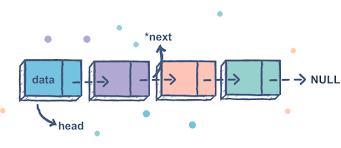
\includegraphics[width=0.6\textwidth]{images/singly-linked-list.png}\\[1cm] 	% University logo
\vfill 
\end{titlepage}

%%%% SECTIONS
%% Section 1
\section{Objectives and Overview}

The objectives of this lab are as follows:
\begin{itemize}
    \item Implement a generic Binary Search Tree class
    \item Gain familiarity with the recursive  methods of creating, accessing, and modifying a binary search tree.
\end{itemize}
This document is organized into two sections. Section~\ref{sec:treenode}
describes the implementation of the individual elements that will make up our
tree, the \lstinline|TreeNode<E>| class. This class will be similar in spirit
to the \lstinline|ListNode<E>| class we implemented when constructing a linked list.
Next, Section~\ref{sec:bst} will describe the implementation of the \lstinline|BinarySearchTree<E>|
class which is responsible for defining the construction of an access to a Binary
Search Tree. You are provided the \lstinline|BinarySearchTree.java| file which contains 
the wrappers and their respective methods stubs.


\section{Step 0: Understanding what you're given} 
\subsection{TreeNode Class }\label{sec:treenode}

The \lstinline|TreeNode<E>| class should be declared as an \textit{inner class}
with respect to the \lstinline|BinarySearchTree<E>| class. This design choice is made for
the same reasons as when we declared \lstinline|ListNode<E>| class as an inner
class in the linked list assignment. Review that assignment document 
regarding this topic for further information.

\subsubsection{Attributes}
The list node has three attributes:
\begin{enumerate}
    \item A generic variable for holding that node's data.
    \item A reference to a \lstinline|TreeNode<E>| on the left.
    \item A reference to a \lstinline|TreeNode<E>| on the right.
\end{enumerate}
It is acceptable to leave each of variables at the default level of access.

\subsubsection{Constructor}
This class has only a single constructor that initializes the data associated
with the node to the data passed in via the constructors parameter. Additionally,
it sets the \lstinline|left| and \lstinline|right| attributes to null.

\subsection{BinarySearchTree Class - Structure and Specs}\label{sec:bst}

Since the \lstinline|TreeNode<E>| is declared as an inner class to the
\lstinline|BinarySearchTree<E>| class this assignment will only involve one
class file.

\subsubsection{Attributes}
This class should have two attributes:
\begin{enumerate}
    \item \lstinline|private TreeNode<E> root|: This variable contains the root of the whole tree. Much like the \lstinline|head| attributes allowed access to the front of the linked list, the \lstinline|root| allows us access to the top of the tree. It is from this point that we will start all of our traversals.
    \item \lstinline|private int size|: An integer containing the current number of nodes in the tree. \textbf{This attribute should be incremented and decremented every time a node is added to removed, respectively.}
\end{enumerate}
In keeping with the design principle of encapsulation be sure to declare
these variables with the access level of \lstinline|private|. We never want 
the user of this class to have to directly intercut with either the root or
the size. Rather, we will define methods that allow this to be abstracted away.

\subsection{Constructors}
This class has a single constructor of the following form: \lstinline|public BinarySearchTree(){ ... }|: This is the basic constructor which initializes the
\lstinline|root| of the tree to \lstinline|null| and \lstinline|size| to 0.


We will begin with Section~\ref{sec:adding} which will detail how to add a node
to a BST. This should be implemented first since we will need to add some nodes
to the BST in order to perform all other methods. Then Section~\ref{sec:ordertraverse}
should be implemented as this provides a method of printing the contents of the tree.
Section~\ref{sec:search} should then be implemented as the \lstinline|findMin| method 
detailed in that section is crucial to implementing the final method you will
implement in Section~\ref{sec:remove}, the remove method. Lastly, you will end
by adding a getter method for the size attribute.


\section{Step 1: Adding and Traversing}

We will begin the BST by implementing the methods for adding and traversing the
tree. The purpose of this is we will need to both add nodes to the tree and
have method of outputting the contents of tree to test future use of the
removal method.

\subsection{Adding a Node}\label{sec:adding}
\begin{minipage}{0.32\textwidth}
    \centering
    \vspace{0.1cm}
    \begin{figure}[H]
    \begin{tikzpicture}[level distance=1.5cm,
        level 1/.style={sibling distance=3cm},
        level 2/.style={sibling distance=1.5cm},
        every node/.style = {minimum width = 2em, draw, circle}
        ]
        \node[fill=!10!orange] {5}
            child {node {3}
                child {node {1}}
                child {node {4}}
            }
            child {node {7}
                child {edge from parent[draw = none] }
                child {node {8}}
            };
    \end{tikzpicture}
    \caption{Current Node is 5 which is less than 6 so we proceed right}
    \label{label:add1}
    \end{figure}
\end{minipage}
\hfill
\begin{minipage}{0.32\textwidth}
    \centering
    \begin{figure}[H]
    \begin{tikzpicture}[level distance=1.5cm,
        level 1/.style={sibling distance=3cm},
        level 2/.style={sibling distance=1.5cm},
        every node/.style = {minimum width = 2em, draw, circle}
        ]
        \node {5}
            child {node {3}
                child {node {1}}
                child {node {4}}
            }
            child {node[fill=!10!orange] {7}
                child {edge from parent[draw = none]}
                child {node {8}}
            };
    \end{tikzpicture}
    \caption{Current node is 7 which is less than 6. The left pointer is null so we can stop traversing and insert here.}
    \label{label:add2}
    \end{figure}
\end{minipage}
\hfill
\begin{minipage}{0.32\textwidth}
    \centering
    \begin{figure}[H]
    \begin{tikzpicture}[level distance=1.5cm,
        level 1/.style={sibling distance=3cm},
        level 2/.style={sibling distance=1.5cm},
        every node/.style = {minimum width = 2em, draw, circle}
        ]
        \node {5}
            child {node {3}
                child {node {1}}
                child {node {4}}
            }
            child {node {7}
                child {node[fill=!10!orange] {6}}
                child {node {8}}
            };
    \end{tikzpicture}
    \caption{The final tree.}
    \label{label:add3}
    \end{figure}
\end{minipage}
\vspace{0.25cm}

Adding a node is very similar to search in that you will use the BST property
to ``search'' for the first available (e.g, \lstinline|null|) spot in the tree.
This process, as displayed in Figure \ref{label:add1}-\ref{label:add3},
involves the following steps: 
\begin{enumerate}
    \item As we are traversing if the data associated with the current node is greater than the node we are attempting to insert and the left pointer is null then insert as that node's left child; otherwise, proceed left.
    \item As we are traversing if the data associated with the current node is less than the node we are attempting to insert and the right pointer is null then insert as that node's left child; otherwise, proceed right.
    \item As we are traversing if the data associated with the current node is equal to the one we are attempting to insert then we can stop traversing as we do not need to insert the node.
\end{enumerate}

\textbf{Your Task:} Implement a method  that takes a generic parameter
\lstinline|data|, instantiates a new \lstinline|TreeNode|  and inserts it into
the tree according to BST insertion rules described above. One of the following
method signatures should be used depending on whether you choose to implement
this iteratively or recursively.
\begin{itemize}
    \item \textbf{Iterative:} \lstinline|public void add(T data){ ... }|
    \item \textbf{Recursive:} \lstinline|public void add(TreeNode<T> curr, T data){ ... }|
\end{itemize}



\subsection{Order Traversals}\label{sec:ordertraverse}
As a review, here are examples of the three types of tree traversals along with
pseudocode for printing all of the nodes in the binary tree:\\
\vspace{0.1cm}
\begin{figure}[H]
    \centering
    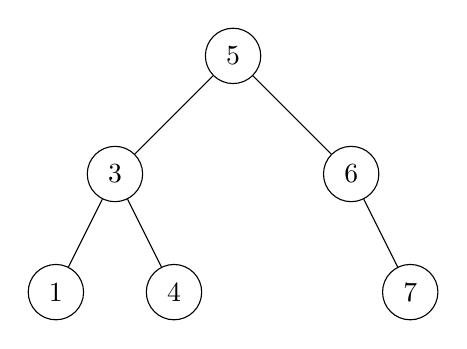
\begin{tikzpicture}[level distance=1.5cm,
        level 1/.style={sibling distance=3cm},
        level 2/.style={sibling distance=1.5cm},
        every node/.style = {minimum width = 2em, draw, circle}
        ]
        \node {5}
            child {node {3}
                child {node {1}}
                child {node {4}}
            }
            child {node {6}
                child {edge from parent[draw = none]}
                child {node {7}}
            };
    \end{tikzpicture}
\end{figure}
\vspace{0.5cm}\\
\begin{minipage}{0.32\textwidth}
\RestyleAlgo{ruled} 
\centering
\begin{algorithm}[H]
    \caption{Inorder}\label{inorder}
    \DontPrintSemicolon
    \SetKwFunction{FInorder}{Inorder}
    \SetKwProg{Fn}{Function}{}{\KwRet}
    \Fn{\FInorder{curr}}{
        \If{curr is null}{
            return\;
        }
        print(node)\;
        Inorder(node.left)\;
        Inorder(node.right)\;
    }
\end{algorithm}
\textbf{Inorder:} 1 3 4 5 6 8
\end{minipage}
\begin{minipage}{0.32\textwidth}
\RestyleAlgo{ruled} 
\centering
\begin{algorithm}[H]
    \caption{Preorder}\label{preorder}
    \DontPrintSemicolon
    \SetKwFunction{FPreorder}{Preorder}
    \SetKwProg{Fn}{Function}{}{\KwRet}
    \Fn{\FPreorder{curr}}{
        \If{curr is null}{
            return\;
        }
        Preorder(node.left)\;
        print(node)\;
        Preorder(node.right)\;
    }
\end{algorithm}
\textbf{Preorder:} 5 3 1 4 6 7
\end{minipage}
\begin{minipage}{0.32\textwidth}
\centering
\RestyleAlgo{ruled} 
\begin{algorithm}[H]
    \caption{Postorder}\label{postorder}
    \DontPrintSemicolon
    \SetKwFunction{FPostorder}{Postorder}
    \SetKwProg{Fn}{Function}{}{\KwRet}
    \Fn{\FPostorder{curr}}{
        \If{curr is null}{
            return\;
        }
        Postorder(node.left)\;
        Postorder(node.right)\;
        print(node)\;
    }
\end{algorithm}
\textbf{Postorder:} 1 4 3 7 6 5
\end{minipage}
\vspace{0.5cm}\\

Printing is relatively straight forward given the ease with which you can
recursively traverse and print nodes from a tree. Your task will be to modify
this approach such that your methods return a list of references to the nodes
in the order of the respective method's traversal. Though this can be done either
iteratively or recursively we will be requiring you to form an iterative solution 
for this set of methods. Consider the details on the differences and similarities
between recursive and iterative traversals of trees at the beginning of the lab
to form this transformation (Section~\ref{sec:traversals}).

\vspace{0.5cm}\\
\textbf{Your Task: } Implement the following methods that use the
aforementioned traversals and return an \lstinline|List| of
references the instances of \lstinline|TreeNode| in the tree.
\begin{enumerate}
    \item \lstinline|public List<TreeNode> getInorderTraversal(){ ... }|
    \item \lstinline|public List<TreeNode> getPostorderTraversal(){ ... }|
    \item \lstinline|public List<TreeNode> getPreorderTraversal(){ ... }|
\end{enumerate}



\newpage

\section{Step 2: Implementing Search}
\subsection{Search}\label{sec:search}
As the name suggests one of the primary methods  of a Binary \textit{Search}
Tree is to provide the ability to \textit{search} for an access a specific node
in the tree. Searching will also form the basis for adding and removing nodes.
In a BST you should keep in mind the following rules:
\begin{enumerate}
    \item For a given root node, the left node is less than the root and the right node is greater than the root.
    \item The leftmost node in a tree contains the smallest value.
    \item The rightmost node in a tree contains the greatest value.
\end{enumerate}
The first of these rules is the one with which we will concern ourselves with
for performing a general search. The latter two can be used to search for the
greatest node or the least node in a tree.\\

\textbf{Your Task: } Using these rules, implement the following methods that
search for nodes in the BST.  These methods can be implemented either
recursively or iteratively. Whichever solution you choose to pursue, do take
care to use the proper method signature as detailed below:
\begin{itemize}
    \item A search method:
    \begin{itemize}
        \item \textbf{Iterative:} \lstinline|public TreeNode<E> search(E data){ ... }|
        \item \textbf{Recursive:} \lstinline|public TreeNode<E> search(TreeNode<E> curr, T data){ ... }|
    \end{itemize}
    \item A method that retrieves the minimum node in a tree:
    \begin{itemize}
        \item \textbf{Iterative:} \lstinline|public TreeNode<E> getMinimum(){ ... }|
        \item \textbf{Recursive:} \lstinline|public TreeNode<E> getMinimum(TreeNode<E> curr){ ... }|
    \end{itemize}
    \item A method that retrieves the maximum node in a tree:
    \begin{itemize}
        \item \textbf{Iterative:} \lstinline|public TreeNode<E> getMaximum(){ ... }|
        \item \textbf{Recursive:} \lstinline|public TreeNode<E> getMaximum(TreeNode<E> curr){ ... }|
    \end{itemize}
\end{itemize}


\newpage
\section{Step 3: Implementing Remove}
\subsection{Removing a Node}\label{sec:remove}
\vspace{0.25cm}\\
\begin{minipage}{0.32\textwidth}
    \centering
    \vspace{0.1cm}
    \begin{figure}[H]
    \begin{tikzpicture}[level distance=1.5cm,
        level 1/.style={sibling distance=3cm},
        level 2/.style={sibling distance=1.5cm},
        every node/.style = {minimum width = 2em, draw, circle}
        ]
        \node {5}
            child {node {3}
                child {node {1}}
                child {node[fill=!10!orange] {4}}
            }
            child {node {6}
                child {edge from parent[draw = none]}
                child {node {8}}
            };
    \end{tikzpicture}
    \caption{Leaf}
    \label{fig:nodeleaf}
    \end{figure}
\end{minipage}
\hfill
\begin{minipage}{0.32\textwidth}
    \centering
    \begin{figure}[H]
    \begin{tikzpicture}[level distance=1.5cm,
        level 1/.style={sibling distance=3cm},
        level 2/.style={sibling distance=1.5cm},
        every node/.style = {minimum width = 2em, draw, circle}
        ]
        \node {5}
            child {node {3}
                child {node {1}}
                child {node {4}}
            }
            child {node[fill=!10!orange] {6}
                child {edge from parent[draw = none]}
                child {node {8}}
            };
    \end{tikzpicture}
    \caption{One Subtree}
    \label{fig:nodeonechild}
    \end{figure}
\end{minipage}
\hfill
\begin{minipage}{0.32\textwidth}
    \centering
    \begin{figure}[H]
    \begin{tikzpicture}[level distance=1.5cm,
        level 1/.style={sibling distance=3cm},
        level 2/.style={sibling distance=1.5cm},
        every node/.style = {minimum width = 2em, draw, circle}
        ]
        \node {5}
            child {node[fill=!10!orange] {3}
                child {node {1}}
                child {node {4}}
            }
            child {node {6}
                child {edge from parent[draw = none]}
                child {node {8}}
            };
    \end{tikzpicture}
    \caption{Two Subtrees}
    \label{fig:nodetwochildren}
    \end{figure}
\end{minipage}
\vspace{0.25cm}\\
Removing a node once again begins with a search, however, once we have found
the node we wish to remove, there are three situations we must consider:
\begin{enumerate}
    \item The node we are removing is a leaf (Figure~\ref{fig:nodeleaf}).
    \item The node we are removing has one subtree(Figure~\ref{fig:nodeonechild}).
    \item The node we are removing has two subtrees (Figure~\ref{fig:nodetwochildren}).
\end{enumerate}

\textbf{Your Task: } Your task will be to create the following method:
\lstinline|public void remove(??){ ... }|. The parameters of this method
 are up to you and the approach you take. A suggested strategy for dealing with
 the various removal cases enumerated above is detailed in the following
 sections.


\newpage

\paragraph{Removing a Leaf}\hfill\\

\vspace{0.25cm}\\
\begin{minipage}{0.49\textwidth}
    \centering
    \vspace{0.1cm}
    \begin{figure}[H]
    \centering
    \begin{tikzpicture}[level distance=1.5cm,
        level 1/.style={sibling distance=3cm},
        level 2/.style={sibling distance=1.5cm},
        every node/.style = {minimum width = 2em, draw, circle}
        ]
        \node {5}
            child {node[fill=blue!70] {\textbf{3}}
                child {node {1}}
                child {node[fill=!10!orange] {4}}
            }
            child {node {6}
                child {edge from parent[draw = none]}
                child {node {8}}
            };
    \end{tikzpicture}
    \caption{Find the node you want to remove (orange), in this case the one with  value 4, and that node's parent (blue)}
    \label{fig:nodeleaf}
    \end{figure}
\end{minipage}
\hfill
\begin{minipage}{0.49\textwidth}
    \centering
    \begin{figure}[H]
    \centering
    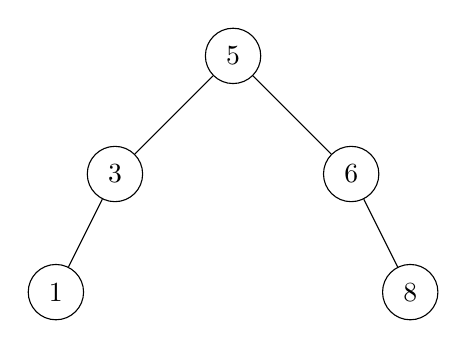
\begin{tikzpicture}[level distance=1.5cm,
        level 1/.style={sibling distance=3cm},
        level 2/.style={sibling distance=1.5cm},
        every node/.style = {minimum width = 2em, draw, circle}
        ]
        \node {5}
            child {node {3}
                child {node {1}}
                child {edge from parent[draw = none]}
            }
            child {node {6}
                child {edge from parent[draw = none]}
                child {node {8}}
            };
    \end{tikzpicture}
    \caption{Set the parent's reference to that node, in this case \lstinline|parent.left| equal to \lstinline|null| to remove the node}
    \label{fig:nodeonechild}
    \end{figure}
\end{minipage}\\
\vspace{0.25cm}\\
The removal of a leaf is perhaps the most straightforward operation. In the
event that both the right and the left points of a node are null then we only
need remove the reference from that node's parent to it.





\paragraph{Removing a Node with One Subtree}\hfill\\

\vspace{0.25cm}\\
\begin{minipage}{0.32\textwidth}
    \centering
    \vspace{0.1cm}
    \begin{figure}[H]
    \begin{tikzpicture}[level distance=1.5cm,
        level 1/.style={sibling distance=3cm},
        level 2/.style={sibling distance=1.5cm},
        every node/.style = {minimum width = 2em, draw, circle}
        ]
        \node[fill=blue!70] {5}
            child {node {3}
                child {node {1}}
                child {node {4}}
            }
            child {node[fill=!10!orange] {6}
                child {edge from parent[draw = none]}
                child {node {8}
                    child {node {7}}
                    child {node {9}}
                }
            };
    \end{tikzpicture}
    \caption{Find the node you want to remove (orange) and that node's parent (blue)}
    \label{fig:onesubtree-1}
    \end{figure}
\end{minipage}
\hfill
\begin{minipage}{0.32\textwidth}
    \centering
    \begin{figure}[H]
    \begin{tikzpicture}[level distance=1.5cm,
        level 1/.style={sibling distance=3cm},
        level 2/.style={sibling distance=1.5cm},
        every node/.style = {minimum width = 2em, draw, circle}
        ]
        \node[fill=blue!70] (P) {5}
            child {node {3}
                child {node {1}}
                child {node {4}}
            }
            child {node[fill=!10!orange] (R) {6}
                child {edge from parent[draw = none]}
                child {node (C) {8}
                    child {node {7}}
                    child {node {9}}
                }
            };
        \draw (P) to [bend left=40] (C);

        % I can't figure out how to remove the edge from the tree so we're 
        % just going to use some "whiteout"
        \foreach \x in {0,...,4}
            \draw[thick, white!100] (P) to (R);
    \end{tikzpicture}
    \caption{Set \lstinline|parent.right| to the root of the node we want to remove's subtree.}
    \label{fig:onesubtree-2}
    \end{figure}
\end{minipage}
\hfill
\begin{minipage}{0.3\textwidth}
    \centering
    \vspace{0.75cm}
    \begin{figure}[H]
    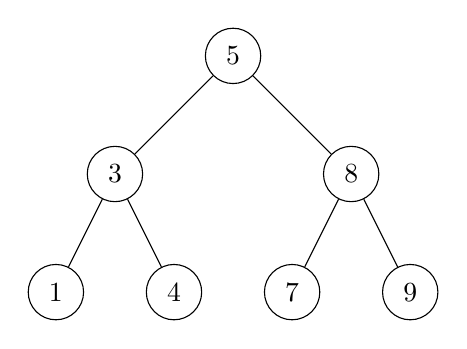
\begin{tikzpicture}[level distance=1.5cm,
        level 1/.style={sibling distance=3cm},
        level 2/.style={sibling distance=1.5cm},
        every node/.style = {minimum width = 2em, draw, circle}
        ]
        \node {5}
            child {node {3}
                child {node {1}}
                child {node {4}}
            }
            child {node {8}
                child {node {7}}
                child {node {9}}
            };
    \end{tikzpicture}
    \vspace{0.9cm}
    \caption{Set the node we  want to remove's reference to it's subtree is \lstinline|null|, thus removing it from the tree}
    \label{fig:onesubtree-3}
    \end{figure}
\end{minipage}
\vspace{0.25cm}\\

The second case, where the node we want to remove has a right or left subtree,
is still relatively straight forward. As with the first step we begin by
finding the node we want to remove and it's parent
(Figure~\ref{fig:onesubtree-1}).  We then take the right pointer of the parent
and short-circut the tree by updating it to point to root of the node we want 
to remove's existing subtree (Figure~\ref{fig:onesubtree-2}). Now, at this point
the node is no longer reachable but it is still attached to the graph. In order
to totally remove it we must set the reference from the node we want to remove
to the root of it's subtree equal to \lstinline|null| (Figure~\ref{fig:onesubtree-3}).


\newpage
\paragraph{Removing a Node with Two Subtrees}\hfill\\

\vspace{0.25cm}\\
\begin{minipage}{0.32\textwidth}
    \centering
    \vspace{0.1cm}
    \begin{figure}[H]
    \begin{tikzpicture}[level distance=1.5cm,
        level 1/.style={sibling distance=3cm},
        level 2/.style={sibling distance=1.5cm},
        level 3/.style={sibling distance=.75cm},
        every node/.style = {minimum width = 2em, draw, circle}
        ]
        \node {5}
            child {node {3}}
            child {node[fill=!10!orange] (R) {10}
                child {node (C) {8}
                    child {node {7}}
                    child {node {9}}
                }
                child {node (C) {12}
                    child {node {11}}
                    child {node {13}}
                }
            };
    \end{tikzpicture}
    \caption{Find the node you want to remove (orange)}
    \label{fig:twosubtrees-0}
    \end{figure}
\end{minipage}
\hfill
\begin{minipage}{0.32\textwidth}
    \centering
    \begin{figure}[H]
    \begin{tikzpicture}[level distance=1.5cm,
        level 1/.style={sibling distance=3cm},
        level 2/.style={sibling distance=1.5cm},
        level 3/.style={sibling distance=.75cm},
        every node/.style = {minimum width = 2em, draw, circle}]
        \node (P) {5}
            child {node {3}}
            child {node[fill=!10!orange] (R) {11}
                child {node {8}
                    child {node {7}}
                    child {node {9}}
                }
                child {node {12}
                    child {node[fill=red!70] (S) {11}}
                    child {node {13}}
                }
            };
        \draw[->, red, thick] (S) -- (R);
    \end{tikzpicture}
    \caption{Find the successor node (red) and copy the successor's value to the node we want to remove.}
    \label{fig:twosubtrees-1}
    \end{figure}
\end{minipage}
\hfill
\begin{minipage}{0.3\textwidth}
    \centering
    \begin{figure}[H]
    \begin{tikzpicture}[level distance=1.5cm,
        level 1/.style={sibling distance=3cm},
        level 2/.style={sibling distance=1.5cm},
        level 3/.style={sibling distance=.75cm},
        every node/.style = {minimum width = 2em, draw, circle}]
        \node (P) {5}
            child {node {3}}
            child {node[fill=!10!orange] (R) {11}
                child {node {8}
                    child {node {7}}
                    child {node {9}}
                }
                child {node {12}
                    child {edge from parent[draw=none]}
                    child {node {13}}
                }
            };
    \end{tikzpicture}
    \caption{Call the removal method on the successor node.}
    \label{fig:twosubtrees-2}
    \end{figure}
\end{minipage}
\vspace{0.25cm}\\

The process of removing a node that has two subtrees begins with finding the
node we want to remove (Figure~\ref{fig:twosubtrees-0}). We then have to find
the minimum node in the node we want to remove's right subtree; otherwise known
as the node we want to remove's ``inorder successor''. At this point the most
straightforward option to ``remove'' the orange node is to copy the data from
the inorder successor node (Figure~\ref{fig:twosubtrees-2}). Finally, we make
a recursive call to the \lstinline|remove| method to remove the successor
node.



\section{Final Step: Getting the size}
\textbf{Your Task:} This class only has one attribute we are interested in and
that is the variable containing the number of nodes in the tree. Create a
getter using the appropriate format that returns that value.


\section{Checklist}

\begin{itemize}
    \item The following accessors and tree modification methods have been implemented:
    \begin{itemize}
        \item[$\square] \lstinline|add| (Section~\ref{sec:adding})
        \item Order traversals implemented iteratively(Section~\ref{sec:ordertraverse})
        \begin{todolist}
            \item \lstinline|traverseInorder|
            \item \lstinline|traversePostorder|
            \item \lstinline|traversePreorder|
        \end{todolist}
        \item Search (Section~\ref{sec:search})
        \begin{todolist}
            \item \lstinline|search|
            \item \lstinline|findMinNode|
        \end{todolist}
        \item[$\square] \lstinline|remove| (Section~\ref{sec:remove})
        \item[$\square$] A getter method for the attribute containing the number of nodes in the tree.
    \end{itemize}
\end{itemize}


%%\newpage
%%\bibliographystyle{apacite}
%%\bibliography{sample}

\end{document}
